\chapter{Limits of Sequences and Filters}

\section{Closure and Interior}
\subsection{Smallest Open Sets and Largest Closed Sets}



\subsubsection{Smallest Open Subset}

We consider the subset~$B ≔ [0, 1]$ of~$ℝ$.
Let~$U$ be any open subset of~$ℝ$ containing~$B$.
Both end points~$0$ and~$1$ are contained in~$U$, so there exist some radii~$ε, δ > 0$ with~$\ball(0, ε) ⊆ U$ and~$\ball(1, δ) ⊆ U$, and~$ε, δ < 1$.
It follows that the set~$U$ contains the open interval~$(-ε, 1 + δ) = \ball(0, ε) ∪ B ∪ \ball(1, δ)$.
It further follows for the radius~$κ ≔ \min(ε, δ) / 2$ that the open interval~$(-κ, 1 + κ)$ is properly contained in~$U$.

This shows that there exists no open subset of~$ℝ$ that is minimal amongst all open subsets of~$ℝ$ that contain~$B$.



\subsubsection{Largest Closed Subset}

We consider the subset~$B ≔ (0, 1)$ of~$ℝ$.
Let~$C$ be any closed subset of~$ℝ$ contained in~$B$.
The elements~$x ≔ \inf C$ and~$\sup C$ are again contained in~$C$, whence~$0 < x, y < 1$.
It follows that the closed interval~$[x, y]$ is contained in~$B$, with~$C$ contained in~$[x, y]$.
Let~$x'$ and~$y'$ be two real numbers with~$0 < x' < x$ and~$y < y' < 1$.
The closed interval~$[x', y']$ is again contained in~$B$, with~$C$ properly contained in~$[x', y']$.

This shows that there exist no closed subset of~$ℝ$ that is maximal amongst all closed subsets of~$ℝ$ that are contained in~$B$.

\subsection{Closure in Terms of Limit Points}

\begin{proposition}
	\label{closure via intersection with neighbourhoods}
	Let~$X$ be a topological space, let~$B$ be a subset of~$X$ and let~$x$ be a point in~$X$.
	The following conditions on~$x$ and~$B$ are equivalent:
	\begin{equivalenceslist}

		\item
			\label{contained in the closure}
			The point~$x$ in contained in the closure of~$B$.

		\item
			\label{every neighbourhood intersects}
			Every neighbourhood of~$x$ intersects~$B$.

		\item
			\label{every open neighbourhood intersects}
			Every open neighbourhood of~$x$ intersects~$B$.

	\end{equivalenceslist}
\end{proposition}

\begin{proof}
	Conditions~\ref{every neighbourhood intersects} and~\ref{every open neighbourhood intersects} are equivalent because every neighbourhood contains an open neighbourhood.
	We have also the chain of equivalences
	\begin{align*}
		{}&
		x ∉ \closure{B} \\
		\iff{}&
		\text{$x ∉ C$ for some closed subset~$C$ of~$X$ with~$B ⊆ C$} \\
		\iff{}&
		\text{$x ∈ U$ for some open subset~$U$ of~$X$ disjoint to~$B$} \\
		\iff{}&
		\text{some open neighbourhood of~$x$ doesn’t intersect~$B$} \,,
	\end{align*}
	which gives the equivalence of Conditions~\ref{contained in the closure} and~\ref{every open neighbourhood intersects}.
\end{proof}

Let~$X$ be a topological space, let~$B$ be a subset of~$X$, and let~$B'$ be the set of limit points of~$B$.
We have for every point~$x$ of~$X$ the chain of equivalences
\begin{align*}
	{}&
	x ∈ \closure{B}
	\\
	\iff{}&
	\text{every open neighbourhood of~$x$ intersects~$B$}
	\\
	\iff{}&
	\left\{
		\begin{tabular}{@{}l}
			every open neighbourhood of~$x$ intersects~$B ∖ \{ x \}$, \\
			or otherwise~$x ∈ B$
		\end{tabular}
	\right.
	\\
	\iff{}&
	\text{$x ∈ B'$ or~$x ∈ B$} \\
	\iff{}&
	x ∈ B' ∪ B \,.
\end{align*}
This shows the claimed equality~$\closure{B} = B' ∪ B$.


\section{Sequences}
\subsection{Theorem~3.3}

For every open neighbourhood~$U$ of~$x$ there exists some index~$N$ with~$x_n ∈ U$ for every~$n ≥ N$.
This entails that~$U$ and~$\{ x_n \suchthat n ≥ 0 \}$ intersect, whence~$U$ and~$A$ intersect.

This shows that every open neighbourhood of~$x$ intersects the set~$A$, which tells us that~$x$ is contained in the closure of~$A$.

\subsection{Theorem~3.4}

Let~$U$ be an open neighbourhood of~$fx$ in~$Y$.
The preimage~$f^{-1} U$ is an open neighbourhood of~$x$ in~$X$.
Because the sequence~$(x_n)_n$ converges to~$x$, there exists some index~$N$ with~$x_n ∈ f^{-1} U$ for every~$n ≥ N$.
Consequently,~$f x_n ∈ U$ for every~$n ≥ N$.

\subsection{Example~3.4}

\begin{lemma}
	\label{uniquess of sequential limits is inherited by finer topologies}
	Let~$X$ be a set and let~$\top{T}_1$ and~$\top{T}_2$ be two topologies on~$X$.
	Suppose that limits of sequences with respect to~$\top{T}_1$ are unique and that the topology~$\top{T}_2$ is finer than the topology~$\top{T}_1$.
\end{lemma}

\begin{proof}
	Let~$(x_n)_n$ be a sequence in~$X$ with limits~$x$ and~$y$ with respect to~$\top{T}_2$.
	Then~$x$ and~$y$ are also limits of~$(x_n)_n$ with respect to~$\top{T}_1$, since~$\top{T}_1$ is coarser than~$\top{T}_2$.
	Consequently,~$x = y$.
\end{proof}

Let~$X$ be the real line together with the cocountable topology.
Every two proper open subsets of~$X$ intersect (because the union of two countable subsets is again a proper subset of~$X$).
Therefore, no two points of~$X$ can be separated by disjoint open neighbourhoods:
the space~$X$ is very much not a Hausdorff space.

Let~$(x_n)_n$ be a sequence in~$X$ that converges to a point~$x$.
We note that the set~$U ≔ X ∖ \{ x_n \suchthat n ≥ 0 \}$ is open in~$X$, and that the sequence~$(x_n)_n$ never enters the set~$U$.
Therefore,~$x$ cannot lie in~$U$.
More generally, every subsequence~$(x_{k_i})_i$ also converges to~$x$, whence~$x$ cannot be contained in~$X ∖ \{ x_{k_i} \suchthat i ≥ 0 \}$.

The point~$x$ must thus be contained in every subsequence of~$(x_n)_n$.
This is only possible if the sequence~$(x_n)_n$ is eventually constant with value~$x$, i.e., if there exists some index~$N$ with~$x_n = x$ for every~$n ≥ N$.

Consequently, the possible limits of the sequence~$(x_n)_n$ are the same as the limits of the constant sequence~$x, x, \dotsc$
The cocountable topology is finer than the cofinite topology, so it follows from Theorem~3.1 (and the above \cref{uniquess of sequential limits is inherited by finer topologies}) that~$x$ is the unique limit of~$(x_n)_n$.

\subsection{Example~3.5}



\subsubsection{General Observations}

Sawtooth functions correspond to sequences of numbers
\[
	0 < s_1 < r_1 < s_2 < r_2 < \dotsb < s_n < r_n < 1 \,,
\]
where~$n ≥ 1$, the numbers~$r_1, \dotsc, r_n$ are the positions of the vertices, and the numbers~$s_1, \dotsc, s_n$ are the positions of the spikes, see \cref{parametrization of sawtooth functions}.
\begin{figure}
	\centering
	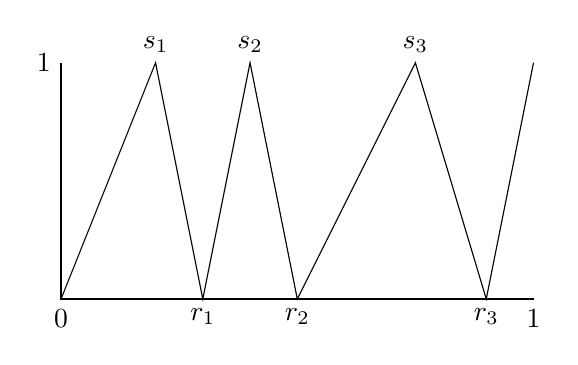
\begin{tikzpicture}[scale = 3, xscale = 2]
		% axis
			\draw[thick] (0, 1) node[left]{$1$} -- (0, 0) node[below]{$0$} -- (1, 0) node[below]{$1$};
		% the line
		\draw (0, 0)
		-- (0.2 , 1) node[above] {$s_1$}
		-- (0.3 , 0) node[below] {$r_1$}
		-- (0.4 , 1) node[above] {$s_2$}
		-- (0.5 , 0) node[below] {$r_2$}
		-- (0.75, 1) node[above] {$s_3$}
		-- (0.9 , 0) node[below] {$r_3$}
		-- (1.0 , 1);
	\end{tikzpicture}
	\caption{Parametrization of sawtooth functions by its vertices and spikes.}
	\label{parametrization of sawtooth functions}
\end{figure}

To describe the closure of~$A$, we will use the following interpolation result.

\begin{proposition}[Interpolation by Sawtooth Functions]
	\label{interpolation via sawtooth functions}
	Let~$n ≥ 1$ be a number of data points, let~$0 < x_1 < \dotsb < x_n < 1$ and let~$y_1, \dotsc, y_n ∈ [0, 1]$.
	There exists a sawtooth function~$f \colon [0, 1] \to [0, 1]$ with~$f x_i = y_i$ for every~$i = 1, \dotsc, n$.
\end{proposition}

\begin{proof}
	Suppose we are given some~$0 < x < 1$ and some~$0 < y < 1$.
	Given~$δ > 0$, there exists a unique line going through the points~$(x - δ, 1)$ and~$(x, y)$.
	This unique line intersects the horizontal line~$ℝ × \{ 1 \}$ at precisely one point, which is of the form~$(x + δ', 0)$ for some~$δ' > 0$, as depicted in \cref{graphical justification for slope formula}.
	We have
	\[
		\frac{y}{δ'} = \frac{1 - y}{δ} \,,
	\]
	and therefore
	\[
		δ' = \frac{y}{1 - y} \, δ \,.
	\]
	\begin{figure}
		\centering
		\begin{tikzpicture}[scale = 3.5, xscale = 1.5];
			% axes
			\draw[thick] (-0.1, 0) node[left] {$0$} -- (1.1, 0);
			\draw[thick] (-0.1, 1) node[left] {$1$} -- (1.1, 1);
			% points
			\draw[fill] (0.2, 1)   ellipse (0.015 and 0.0225) node[above] {$\rightarrow$};
			\draw[fill] (0.5, 0.4) ellipse (0.015 and 0.0225);
			\draw[fill] (0.7, 0)   ellipse (0.015 and 0.0225) node[below] {$\leftarrow$};
			% lines
			\draw (0.5, 0) --node[left] {$y$} (0.5, 0.4) --node[right] {$1 - y$}  (0.5, 1) node[above] {$x$};
			\draw (0.7, 0) -- (0.2, 1);
			% non-visible lines for placement of deltas
			\draw (0.2, 1) --node[above] {$δ$}  (0.5, 1);
			\draw (0.5, 0) --node[below] {$δ'$} (0.7, 0);
		\end{tikzpicture}
		\caption{We have~$y / δ = (1 - y) / δ'$, and as~$δ \to 0$ we also have~$δ' \to 0$.}
		\label{graphical justification for slope formula}
	\end{figure}
	So for~$δ \to 0$ we have also~$δ' \to 0$.

	Let now~$ε > 0$ such that the intervals~$(x_i - ε, x_i + ε)$ are contained in~$[0, 1]$ and pairwise disjoint.
	We define the values~$s_i$ and~$r_i$ as follows:
	\begin{casedistinction}

		\item
			If~$y_i = 0$ then~$s_i ≔ (x_i - ε/2, 1)$ and~$r_i ≔ (x_i, 0) = (x_i, y_i)$.

		\item
			If~$y_i = 1$ then~$s_i ≔ (x_i, 1) = (x_i, y_i)$ and~$r_i ≔ (x_i  + ε/2, 0)$.

		\item
			If~$0 < y_i < 1$, then let~$δ > 0$ be sufficiently small so that both~$δ < ε$ and also~$δ' < ε$ for~$δ' ≔ y / (y - 1) ⋅ δ$.
			We then set~$s_i ≔ (x_i - δ, 1)$ and~$r_i ≔ (x_i + δ', 0)$.

	\end{casedistinction}
	The sawtooth function~$f$ corresponding to the numbers
	\[
		0 < s_1 < r_1 < \dotsb < s_n < r_n < 1
	\]
	satisfies~$f x_i = y_i$ for every~$i = 1, \dotsc, n$.
	See \cref{interpolationg sawtooth function} for an example.
	\begin{figure}
		\[
			\begin{array}{crcr}
				{}
				&
				\centerbox{
				\begin{tikzpicture}[scale = 2.5, xscale = 2]
					% gray areas
					%\draw[fill, gray!30] (0.1, 1) rectangle (0.3, 0);
					%\draw[fill, gray!30] (0.4, 1) rectangle (0.6, 0);
					%\draw[fill, gray!30] (0.7, 1) rectangle (0.9, 0);
					% axes
					\draw[thick] (0, 1) -- (0, 0) -- (1, 0);
					% the points to be interpolated
					\draw[fill] (0.2, 0)   ellipse (0.015 and 0.03);
					\draw[fill] (0.5, 0.5) ellipse (0.015 and 0.03);
					\draw[fill] (0.8, 1)   ellipse (0.015 and 0.03);
					% the intervals with ε = 0.1
					%\draw[(-)] (0.1, -0.2) -- (0.3, -0.2);
					%\draw[(-)] (0.4, -0.2) -- (0.6, -0.2);
					%\draw[(-)] (0.7, -0.2) -- (0.9, -0.2);
				\end{tikzpicture}
				}
				&
				\leadsto
				&
				\centerbox{
				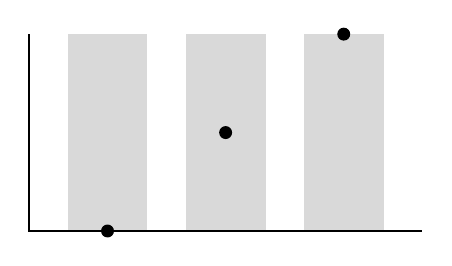
\begin{tikzpicture}[scale = 2.5, xscale = 2]
					% gray areas
					\draw[fill, gray!30] (0.1, 1) rectangle (0.3, 0);
					\draw[fill, gray!30] (0.4, 1) rectangle (0.6, 0);
					\draw[fill, gray!30] (0.7, 1) rectangle (0.9, 0);
					% axes
					\draw[thick] (0, 1) -- (0, 0) -- (1, 0);
					% the points to be interpolated
					\draw[fill] (0.2, 0)   ellipse (0.015 and 0.03);
					\draw[fill] (0.5, 0.5) ellipse (0.015 and 0.03);
					\draw[fill] (0.8, 1)   ellipse (0.015 and 0.03);
					% the intervals with ε = 0.1
					%\draw[(-)] (0.1, -0.2) -- (0.3, -0.2);
					%\draw[(-)] (0.4, -0.2) -- (0.6, -0.2);
					%\draw[(-)] (0.7, -0.2) -- (0.9, -0.2);
				\end{tikzpicture}
				}
				\\[5em]
				\leadsto
				&
				\centerbox{
				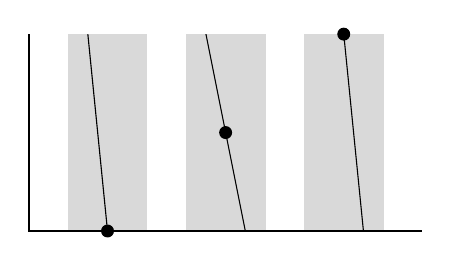
\begin{tikzpicture}[scale = 2.5, xscale = 2]
					% gray areas
					\draw[fill, gray!30] (0.1, 1) rectangle (0.3, 0);
					\draw[fill, gray!30] (0.4, 1) rectangle (0.6, 0);
					\draw[fill, gray!30] (0.7, 1) rectangle (0.9, 0);
					% axes
					\draw[thick] (0, 1) -- (0, 0) -- (1, 0);
					% the points to be interpolated
					\draw[fill] (0.2, 0)   ellipse (0.015 and 0.03);
					\draw[fill] (0.5, 0.5) ellipse (0.015 and 0.03);
					\draw[fill] (0.8, 1)   ellipse (0.015 and 0.03);
					% the intervals with ε = 0.1
					%\draw[(-)] (0.1, -0.2) -- (0.3, -0.2);
					%\draw[(-)] (0.4, -0.2) -- (0.6, -0.2);
					%\draw[(-)] (0.7, -0.2) -- (0.9, -0.2);
					% lines
					\draw (0.15, 1) -- (0.2,  0);
					\draw (0.45, 1) -- (0.55, 0);
					\draw (0.8,  1) -- (0.85, 0);
				\end{tikzpicture}
				}
				&
				\leadsto
				&
				\centerbox{
				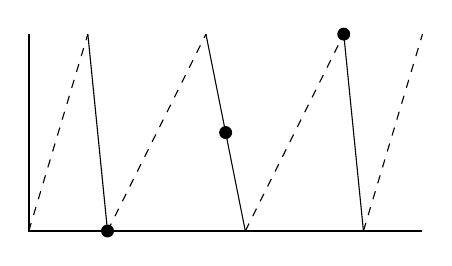
\begin{tikzpicture}[scale = 2.5, xscale = 2]
					% gray areas
					%\draw[fill, gray!30] (0.1, 1) rectangle (0.3, 0);
					%\draw[fill, gray!30] (0.4, 1) rectangle (0.6, 0);
					%\draw[fill, gray!30] (0.7, 1) rectangle (0.9, 0);
					% axes
					\draw[thick] (0, 1) -- (0, 0) -- (1, 0);
					% the points to be interpolated
					\draw[fill] (0.2, 0)   ellipse (0.015 and 0.03);
					\draw[fill] (0.5, 0.5) ellipse (0.015 and 0.03);
					\draw[fill] (0.8, 1)   ellipse (0.015 and 0.03);
					% the intervals with ε = 0.1
					%\draw[(-)] (0.1, -0.2) -- (0.3, -0.2);
					%\draw[(-)] (0.4, -0.2) -- (0.6, -0.2);
					%\draw[(-)] (0.7, -0.2) -- (0.9, -0.2);
					% lines
					\draw (0.15, 1) -- (0.2,  0);
					\draw (0.45, 1) -- (0.55, 0);
					\draw (0.8,  1) -- (0.85, 0);
					\draw[dashed] (0,    0) -- (0.15, 1);
					\draw[dashed] (0.2,  0) -- (0.45, 1);
					\draw[dashed] (0.55, 0) -- (0.8,  1);
					\draw[dashed] (0.85, 0) -- (1,    1);
				\end{tikzpicture}
				}
			\end{array}
		\]
		\caption{A sawtooth function that interpolated between for the three points~$(0.2, 0)$,~$(0.5, 0.5)$ and~$(0.8, 1)$.}
		\label{interpolationg sawtooth function}
	\end{figure}
\end{proof}



\subsubsection{The Closure of~$A$}

Instead of only showing that the zero function lies in the closure in~$A$, we show more generally that~$A$ is dense in~$X$.
To this end, we characterize dense subsets in terms of their intersection with open sets:

\begin{lemma}
	Let~$X$ be a topological space and let~$D$ be a subset of~$X$.
	The set~$D$ is dense in~$X$ if and only if every nonempty open subset of~$X$ intersects~$D$.
\end{lemma}

In other words:
the definition of \enquote{dense} we gave in \cref{definition of dense subsets} is equivalent to the definition given in Section~3.1 the book.

\begin{proof}
	We have the chain of equivalences
	\begin{align*}
		{}&
		\text{$D$ is dense in~$X$} \\
		\iff{}&
		\closure{D} = X \\
		\iff{}&
		\text{the only closed subset of~$X$ that contains~$D$ is~$X$ itself} \\
		\iff{}&
		\text{the only open subset of~$X$ that doesn’t intersect~$D$ is~$∅$} \,,
	\end{align*}
	which proves the assertion.
\end{proof}

Let now~$U$ be any nonempty open subset of~$[0, 1]^{[0, 1]}$.
We need to show that~$A$ intersects~$U$.
For this, we may assume that~$U$ is a basic open set for the product topology, i.e., that there exist distinct points~$x_1, \dotsc, x_n$ in~$[0, 1]$ and open subsets~$U_1, \dotsc, U_n$ of~$[0, 1]$ with
\[
	U
	=
	\{
		f ∈ [0, 1]^{[0, 1]}
		\suchthat
		\text{$f x_i ∈ U_i$ for every~$i$}
	\} \,.
\]
The neighbourhood~$U$ is nonempty, so the sets~$U_i$ must also be nonempty.
For every index~$i$ we choose some point~$y_i$ in~$U_i$.
We know from \cref{interpolation via sawtooth functions} that there exist a sawtooth function~$f$ with~$f x_i = y_i$ for every~$i$, and thus~$f ∈ U$.
This shows that~$U$ intersects~$A$.



\subsubsection{The Zero Function is Not The Limit of a Sequence in~$A$}

\begin{proposition}
	\label{convergece of sequences in products is coordinate-wise}
	Let~$(X_α)_{α ∈ A}$ be a family of topological spaces, let~$(x_n)_n$ be a sequence in~$X ≔ ∏_{α ∈ A} X_α$, and let~$x$ be some point in~$X$.
	Then~$(x_n)_n \to x$ in~$X$ if and only if this holds in each coordinate.
	More explicitly, if~$x_n = (x_n^α)_α$ and~$x = (x^α)_α$, then~$(x_n)_n \to x$ if and only if~$(x_n^α)_α \to x^α$ for every index~$α ∈ A$.
\end{proposition}

\begin{proof}
	For all distinct indices~$α_1, \dotsc, α_r ∈ A$ and all open subsets~$U_i ⊆ X_{α_i}$ we denote the resulting basic open subset of~$X$ by
	\[
		P(U_1, \dotsc, U_r)
		≔
		∏_{α ∈ A}
		\begin{cases*}
			U_i & if~$α = α_i$ for some~$i$, \\
			X_α & otherwise.
		\end{cases*}
	\]
	We have the chain of equivalences
	\begingroup
	\allowdisplaybreaks
	\begin{align*}
		{}&
		(x_n)_n \to x
		\\
		\iff{}&
		\left\{
		\begin{tabular}{l}
			for every open subset~$U$ of~$X$ with~$x ∈ U$, \\
			there exists some~$N$ with~$x_n ∈ U$ for every~$n ≥ N$
		\end{tabular}
		\right.
		\\
		\iff{}&
		\left\{
		\begin{tabular}{l}
			for every basic open subset~$U$ of~$X$ with~$x ∈ U$, \\
			there exists some~$N$ with~$x_n ∈ U$ for every~$n ≥ N$
		\end{tabular}
		\right.
		\\
		\iff{}&
		\left\{
		\begin{tabular}{l}
			for all distinct indices~$α_1, \dotsc, α_r ∈ A$ \\
			and open subsets~$U_i ⊆ X_{α_i}$ with~$x ∈ P(U_1, \dotsc, U_r)$, \\
			there exists some~$N$ with~$x_n ∈ P(U_1, \dotsc, U_r)$ for every~$n ≥ N$
		\end{tabular}
		\right.
		\\
		\iff{}&
		\left\{
		\begin{tabular}{l}
			for all distinct indices~$α_1, \dotsc, α_r ∈ A$ \\
			and open subsets~$U_i ⊆ X_{α_i}$ with~$x^{α_i} ∈ U_i$ for every~$i$, \\
			there exists some~$N$ with~$x_n^{α_i} ∈ U_i$ for all~$i$ and~$n ≥ N$
		\end{tabular}
		\right.
		\\
		\iff{}&
		\left\{
		\begin{tabular}{l}
			for all distinct indices~$α_1, \dotsc, α_r ∈ A$ \\
			and open subsets~$U_i ⊆ X_{α_i}$ with~$x^{α_i} ∈ U_i$ for every~$i$, \\
			there exists some~$N_1, \dotsc, N_r$ with~$x_n^{α_i} ∈ U_i$ for all~$i$ and ~$n ≥ N_i$
		\end{tabular}
		\right.
		\\
		\iff{}&
		\left\{
		\begin{tabular}{l}
			for every index~$α ∈ A$ \\
			and every open subset~$U ⊆ X_α$ with~$x^α ∈ U$, \\
			there exists some~$N$ with~$x_n^α ∈ U$ for every~$n ≥ N$
		\end{tabular}
		\right.
		\\
		\iff{}&
		\text{$(x_n^α)_n \to x^α$ for every~$α ∈ A$} \,.
	\end{align*}
	\endgroup
	This shows the claimed equivalence.
\end{proof}

Suppose there exists a sequence of sawtooth functions~$(f_n)_n$ with~$(f_n)_n \to 0$ with respect to the product topology on~$[0, 1]^{[0, 1]}$.
According to the above \lcnamecref{convergece of sequences in products is coordinate-wise} this is equivalent to~$(f_n)_n \to 0$ pointwise.
However, we will see in the following that this cannot happen, since sawtooth functions are rather rigid:
not too many values of~$f_n$ can tend to~$0$ at the same time.

There exists by assumption for every point~$x$ in~$[0, 1]$ some natural number~$N$ such that~$f_n x ≤ 1/2$ for every~$n ≥ N$.
For every natural number~$N$ let
\[
	B_N
	≔
	\{ x ∈ [0, 1] \suchthat \text{$f_n x ≤ 1/2$ for every~$n ≥ N$} \} \,.
\]
These sets~$B_N$ form an increasing filtration of~$[0, 1]$, i.e., we have
\[
	B_0 ⊆ B_1 ⊆ B_2 ⊆ B_3 ⊆ \dotsb
\]
and~$[0, 1] = ⋃_{N = 0}^∞ B_N$.
We can also describe the sets~$B_N$ in terms of the sets
\[
	B'_n ≔ \{ x ∈ [0, 1] \suchthat f_n x ≤ 1/2 \}
\]
as the intersection~$B_N = ⋂_{n ≥ N} B'_n$.

We note that each set~$B'_n$ is Lebesgue-measurable, since the sawtooth function~$f_n$ is continuous.
Let us calculate the Lebesgue-measure of~$B'_n$:

We observe that for every sawtooth function~$f$ with corresponding points
\[
	0 < s_1 < r_1 < s_2 < r_2 < \dotsb < s_n < r_n < 1 \,,
\]
we have for the set~$B' ≔ \{ x ∈ [0, 1] \suchthat f x ≤ 1/2 \}$ the explicit description
\[
	B'
	=
	\biggl[ 0, \frac{s_1}{2} \biggr]
	∪ \biggl[ \frac{s_1 + r_1}{2}, \frac{r_1 + s_2}{2} \biggr]
	∪ \biggl[ \frac{s_2 + r_2}{2}, \frac{r_2 + s_3}{2} \biggr]
	∪ \dotsb
	∪ \biggl[ \frac{s_n + r_n}{2}, \frac{r_n + 1}{2} \biggr] \,.
\]
See \cref{cutting sawtooth function in half} for a visualization.
\begin{figure}
	\centering
	\begin{tikzpicture}[scale = 3, xscale = 4]
		% coordinates
		\coordinate (0)  at (0,    0);
		\coordinate (s1) at (0.2,  0);
		\coordinate (r1) at (0.3,  0);
		\coordinate (s2) at (0.4,  0);
		\coordinate (r2) at (0.5,  0);
		\coordinate (s3) at (0.75, 0);
		\coordinate (r3) at (0.9,  0);
		% coloured areas
		\draw[fill, gray!50] (0, 0) -- (0.1, 0.5) -- (0.1, 0) -- cycle;
		\draw[fill, gray!50] (0.25, 0) -- (0.25, 0.5) -- (r1) -- (0.35, 0.5) -- (0.35, 0) -- cycle;
		\draw[fill, gray!50] (0.45, 0) -- (0.45, 0.5) -- (r2) -- (0.625, 0.5) -- (0.625, 0) -- cycle;
		\draw[fill, gray!50] (0.825, 0) -- (0.825, 0.5) -- (r3) -- (0.95, 0.5) -- (0.95, 0) -- cycle;
		% the nodes and dashed lines
		\draw[dashed, thick] (0, 1.05) -- ++(0, -1.1) node[below] {$0$};
		\draw[dashed, thick] ($(s1) + (0, 1.05)$) -- ++(0, -1.1) node[below] {$s_1$};
		\draw[dashed, thick] ($(r1) + (0, 1.05)$) -- ++(0, -1.1) node[below] {$r_1$};
		\draw[dashed, thick] ($(s2) + (0, 1.05)$) -- ++(0, -1.1) node[below] {$s_2$};
		\draw[dashed, thick] ($(r2) + (0, 1.05)$) -- ++(0, -1.1) node[below] {$r_2$};
		\draw[dashed, thick] ($(s3) + (0, 1.05)$) -- ++(0, -1.1) node[below] {$s_3$};
		\draw[dashed, thick] ($(r3) + (0, 1.05)$) -- ++(0, -1.1) node[below] {$r_3$};
		\draw[dashed, thick] (1, 1.05) -- ++(0, -1.1) node[below] {$1$};
		% vertical dashed lines
		\draw[dashed, gray!50] (0.1 ,  1.05) -- (0.1,   0);
		\draw[dashed, gray!50] (0.25,  1.05) -- (0.25,  0);
		\draw[dashed, gray!50] (0.35,  1.05) -- (0.35,  0);
		\draw[dashed, gray!50] (0.45,  1.05) -- (0.45,  0);
		\draw[dashed, gray!50] (0.45,  1.05) -- (0.45,  0);
		\draw[dashed, gray!50] (0.625, 1.05) -- (0.625, 0);
		\draw[dashed, gray!50] (0.825, 1.05) -- (0.825, 0);
		\draw[dashed, gray!50] (0.95 , 1.05) -- (0.95 , 0);
		% horizontal dashed lines
		%\draw[dashed, gray!50] (-0.02, 0.5) -- (1.02, 0.5);
		% axis
		\draw[thick] (0, 1) node[left]{$1$} -- (0, 0) -- (1, 0);
		% the line
		\draw (0) -- ($(s1) + (0, 1)$) -- (r1) -- ($(s2) + (0, 1)$) -- (r2) -- ($(s3) + (0, 1)$) -- (r3) -- (1.0 , 1);
	\end{tikzpicture}
	\caption{An explicit description of those points~$x$ with~$f x ≤ 1 / 2$.
	The graph is a triangle in each interval~$[0, s_1], [s_1, r_1], \dotsc, [r_3, 1]$, so we take half of each interval.}
	\label{cutting sawtooth function in half}
\end{figure}
It follows that
\[
	λ B'
	=
	\frac{s_1}{2} + \frac{s_2 - s_1}{2} + \frac{s_3 - s_2}{2} + \dotsb + \frac{1 - s_n}{2}
	=
	\frac{1}{2} \,.
\]
We find in particular that
\[
	λ B'_n = \frac{1}{2}
\]
for every~$n$.

We find now that on the one hand
\[
	λ B_N ≤ λ B'_N ≤ \frac{1}{2}
\]
for every~$N$.
But since the sets~$B_N$ form an increasing filtration of~$[0, 1]$, we also find on the other hand
\[
	λ B_N \to λ [0, 1] = 1 \,.
\]
This is a contradiction!

\subsection{Example~3.6}

We will verify this example in \nameref{exercise 3.6}.

\subsection{Example~3.9}

There is nothing to verify here, since this is the \emph{definition} of a topological manifold.

\subsection{Theorem~3.5}

The presented proof of Theorem~3.5 can be streamlined thanks to the following observation(s).

\begin{proposition}
	Let~$X$ be a topological space and let~$x$ be a point in~$X$ admitting a countable neighbourhood basis~$\{ U_n \suchthat n ≥ 0 \}$.
	For every~$n ≥ 0$ let~$V_n = U_1 ∩ \dotsb ∩ U_n$.
	Then~$\{ V_n \suchthat n ≥ 0 \}$ is again a neighbourhood basis of~$x$.
\end{proposition}

\begin{proof}
	The sets~$V_n$ are again open neighbourhoods of~$x$, since each~$U_n$ is an open neighbourhood of~$x$.
	There exists for every neighbourhood~$U$ of~$x$ some index~$n$ with~$U_n ⊆ U$.
	We have~$V_n ⊆ U_n$, and therefore~$V_n ⊆ U$.
\end{proof}

\begin{corollary}
	\label{first countable spaces have linearly ordered neighbourhood bases}
	Let~$X$ be a first countable topological space.
	Every point~$x$ in~$X$ admits a countable neighbourhood basis~$\{ U_n \suchthat n ≥ 0 \}$ such that~$U_{n + 1} ⊆ U_n$ for every~$n ≥ 0$.
	\qed
\end{corollary}

In the presented proof of Theorem~3.5 we may additionally assume that
\[
	U_0 ⊇ U_1 ⊇ U_2 ⊇ U_3 ⊇ \dotsb
	\quad\text{and}\quad
	V_0 ⊇ V_1 ⊇ V_2 ⊇ V_3 ⊇ \dotsb \,.
\]
This then implies that the sequence~$(x_n)_n$ itself converges to both~$x$ and~$y$.
There is hence no need for subsequences.

\subsection{Theorem~3.6}

In view of Theorem~3.3, it remains to show that for every point~$x$ in~$\closure{A}$ there exists a sequence~$(x_n)_n$ in~$A$ with~$(x_n)_n \to x$.

Let~$\{ U_n \suchthat n ≥ 0 \}$ be a countable neighbourhood basis of~$x$ with
\[
	U_0 ⊇ U_1 ⊇ U_2 ⊇ U_3 ⊇ \dotsb \,,
\]
which exists by \cref{first countable spaces have linearly ordered neighbourhood bases} (page~\pageref{first countable spaces have linearly ordered neighbourhood bases}).
Each open neighbourhood~$U_n$ intersects the set~$A$ because~$x$ is in the closure of~$A$ (by \cref{closure via intersection with neighbourhoods}, page~\pageref{closure via intersection with neighbourhoods}).
There hence exists for every index~$n$ some point~$x_n$ in the intersection~$U_n ∩ A$.

The sequence~$(x_n)_n$ lies completely in~$A$.
There exists for every neighbourhood~$V$ of~$x$ some index~$N$ with~$U_N ⊆ V$.
We then have~$x_n ∈ U_n ⊆ U_N ⊆ V$ for every~$n ≥ N$.
This shows that the sequence~$(x_n)_n$ converges to~$x$.


\subsection{Theorem~3.7}

In view of Theorem~3.4 it remains to show that if the map~$f$ preserves convergence of sequences, then it is continuous.
To this end, we show that for every closed subset~$C$ of~$Y$ its preimage~$f^{-1} C$ is closed in~$X$.

Let~$(x_n)_n$ be a sequence in~$f^{-1} C$ with~$(x_n)_n \to x$ for some point~$x ∈ X$.
Then~$(f x_n)_n \to f x$ and the sequence~$(f x_n)_n$ lies completely in~$C$.
It follows from Theorem~3.6 (and Theorem~3.3) that~$f x$ also lies in~$C$.
Therefore,~$x$ lies in~$f^{-1} C$.
According to Theorem~3.6 we have shown that~$f^{-1} C$ is closed in~$X$.


\section{Filters and Convergence}
\subsection{Generated Filters and Filterbases}

\begin{proposition}
	Let~$X$ be a set and let~$(\filter{F}_α)_{α ∈ A}$ be a family of filters on~$X$.
	The intersection~$⋂_{α ∈ A} \filter{F}_α$ is again a filter on~$X$.
\end{proposition}

\begin{proof}
	We denote the intersection~$⋂_{α ∈ A} \filter{F}_α$ by~$\filter{F}$.

	Let~$A$ and~$B$ be two sets belonging to~$\filter{F}$.
	This means that both~$A$ and~$B$ are contained in each~$\filter{F}_α$.
	Consequently, the intersection~$A ∩ B$ is again contained in each~$\filter{F}_α$.
	Therefore,~$A ∩ B$ is contained in~$\filter{F}$.

	Each~$\filter{F}_α$ is nonempty and upwards closed, and thus contains the set~$X$.
	Therefore,~$X$ is also contained in~$\filter{F}$.
	This shows that~$\filter{F}$ is nonempty.

	Let~$A$ be any set belonging to~$\filter{F}$ and let~$B$ be any subset of~$X$ with~$A ⊆ B$.
	The set~$A$ belongs to each~$\filter{F}_α$, so~$B$ belongs to each~$\filter{F}_α$.
	Hence,~$B$ belongs to~$\filter{F}$.
\end{proof}

\begin{corollary}
	Let~$X$ be a set and let~$\filterbase{S}$ be a collection of subsets of~$X$, i.e., a subset of the power set~$2^X$.
	There exists a smallest filter on~$X$ containing~$\filterbase{S}$.
	\qed
\end{corollary}

\begin{definition}
	Let~$X$ be a set and let~$\filterbase{S}$ be a collection of subsets of~$X$.
	The smallest filter on~$X$ containing~$\filterbase{S}$ is the \defemph{filter generated by~$\filterbase{S}$}.
\end{definition}

\begin{proposition}
	Let~$X$ be a set and let~$\filterbase{B}$ be a collection of subsets of~$X$.
	Suppose that~$\filterbase{B}$ is nonempty and downwards directed.
	Then the filter~$\filter{F}$ generated by~$\filterbase{B}$ is given by
	\[
		\{
			A ⊆ X
			\suchthat
			\text{there exists~$B ∈ \filterbase{B}$ with~$B ⊆ A$}
		\} \,.
	\]
\end{proposition}

\begin{proof}
	We denote the proposed set by~$\filter{G}$.
	The filter~$\filter{F}$ contains~$\filterbase{B}$ and is upwards closed, and therefore also contains~$\filter{G}$, i.e.,~$\filter{G} ⊆ \filter{F}$.
	To prove the inclusion~$\filter{F} ⊆ \filter{G}$ we will show that~$\filter{G}$ is a filter.

	Let~$A$ and~$A'$ be two sets belonging to~$\filter{G}$.
	This means that there exist two sets~$B$ and~$B'$ belonging to~$\filterbase{B}$ with~$B ⊆ A$ and~$B' ⊆ A'$.
	There exists by assumption a set~$B''$ belonging to~$\filterbase{B}$ with~$B'' ⊆ B ∩ B'$, and thus~$B'' ⊆ A ∩ A'$.
	The intersection~$A ∩ A'$ therefore again belongs to~$\filter{G}$.

	There exists some set belonging to~$\filterbase{B}$, whence the set~$X$ belongs to~$\filter{G}$.
	Therefore,~$\filter{G}$ is nonempty.

	Let~$A$ be a set belonging to~$\filter{G}$ and let~$A'$ be a subset of~$X$ with~$A ⊆ A'$.
	There exist some set~$B$ belonging to~$\filterbase{B}$ with~$B ⊆ A$, and thus~$B ⊆ A'$.
	Therefore,~$A'$ again belongs to~$\filter{G}$.
\end{proof}

\begin{proposition}
	Let~$X$ be a set and let~$\filterbase{S}$ be a collection of subsets of~$X$.
	Let~$\filter{F}$ be the filter generated by~$\filterbase{S}$.
	A filterbase for~$\filter{F}$ is given by the collection of finite intersections of sets belonging to~$\filterbase{S}$.
\end{proposition}

\begin{proof}
	Let
	\[
		\filterbase{B}
		≔
		\{
			A_1 ∩ \dotsb ∩ A_n
			\suchthat
			n ≥ 0,
			A_1, \dotsc, A_n ∈ \filterbase{S}
		\}
	\]
	and let~$\filter{F}'$ be the filter generated by~$\filterbase{B}$.
	We have~$\filterbase{S} ⊆ \filterbase{B} ⊆ \filter{F}'$ and thus~$\filter{F} ⊆ \filter{F}'$, because~$\filter{F}'$ is a filter.
	It follows from the inclusion~$\filterbase{S} ⊆ \filter{F}$ that also~$\filterbase{B} ⊆ \filter{F}$, since~$\filter{F}$ is a filter, and therefore~$\filter{F}' ⊆ \filter{F}$, again because~$\filter{F}$ is a filter.
\end{proof}

\subsection{Filters as Homomorphisms}

Let~$𝟚 ≔ \{ 0 < 1 \}$.

We can see that the given statement cannot be correct:
both constant maps from~$2^X$ to~$𝟚$ satisfy the given definition of a homomorphism of meet-semilattice, but the homomorphism with constant value~$0$ corresponds to the empty collection of subsets of~$X$, which is not a filter.

The source of this problem is that the given definition of a meet-semilattice is not correct (for our purposes):
we also need the existence of a greatest element.

\begin{definition}
	A poset~$S$ is a \defemph{meet-semilattice} if
	\begin{enumerate*}
%
		\item
			every two elements of~$S$ admit a meet, and
%
		\item
			the poset~$S$ admits a greatest element.

	\end{enumerate*}
	The meet of two elements~$x$ and~$y$ of~$S$ is denoted by~$x ∧ y$.
	The greatest element of~$S$ is denoted by~$1$ (or by~$⊤$), so that~$x ∧ 1 = x$ for every~$x ∈ S$.
\end{definition}

\begin{definition}
	Let~$S$ and~$T$ be two meet-semilattices.
	A map~$f$ from~$S$ to~$T$ is a \defemph{homomorphism of meet-semilattices} if~$f (x ∧ y) = (f x) ∧ (f y)$ for all~$x, y ∈ X$ and also~$f 1_S = 1_T$.
\end{definition}

\begin{definition}
	Let~$P$ and~$Q$ be two posets.
	A map~$f$ from~$P$ to~$Q$ is \defemph{isotone} if~$f x ≤ f y$ for all~$x, y ∈ P$ with~$x ≤ y$.
\end{definition}

\begin{proposition}
	Every homomorphism of meet-semilattices is isotone.
\end{proposition}

\begin{proof}
	Let~$S$ and~$T$ be two meet-semilattices and let~$f$ be a homomorphism of meet-semilattices from~$S$ to~$T$.
	For every two elements~$x$ and~$y$ of~$S$ we have the chain of equivalences and implications
	\[
		x ≤ y
		\iff
		x ∧ y = x
		\implies
		(f x) ∧ (f y) = f x
		\iff
		f x ≤ f y \,.
	\]
	This shows that~$f$ is isotone.
\end{proof}

\begin{definition}
	Let~$S$ be a meet-semilattice.
	A subset of~$S$ in a \defemph{filter} if it is nonempty, downward directed and upward closed.
\end{definition}

\begin{proposition}
	Let~$S$ be a meet-semilattice.
	A subset~$F$ of~$S$ is a filter if and only if~$1 ∈ F$ and if we have for every two elements~$x$ and~$y$ of~$S$ the equivalence
	\[
		x ∧ y ∈ F \iff \text{$x ∈ F$ and~$y ∈ F$} \,.
	\]
\end{proposition}

\begin{proof}
	Suppose that~$F$ is a filter.
	This entails that~$F$ is upward closed and nonempty, whence~$1$ is contained in~$F$.
	If~$x ∧ y ∈ F$ then also~$x ∈ F$ and~$y ∈ F$ because~$F$ is upward closed.
	If on the other hand~$x ∈ F$ and~$y ∈ F$ then~$x ∧ y ∈ F$ because~$F$ is downward directed and upward closed.

	Suppose not that~$1 ∈ F$ and that for every two elements~$x$ and~$y$ of~$F$, we have~$x ∧ y ∈ F$ if and only if~$x, y ∈ F$.
	We know from the condition~$1 ∈ F$ that~$F$ is nonempty, and the implication~$x, y ∈ F \implies x ∧ y ∈ F$ tells us that~$F$ is downward directed.
	Given~$x ∈ F$ and~$y ∈ S$ with~$x ≤ y$, we have~$x ∧ y = x ∈ F$ and therefore also~$y ∈ F$.
\end{proof}

Let~$S$ be a meet-semilattice.
We know that subsets of~$S$ correspond to maps from~$S$ to~$𝟚$.
More explicitly, for every subset~$F$ of~$S$, the corresponding function~$f$ is given by
\[
	f x
	=
	\begin{cases*}
		1 & if~$x ∈ F$, \\
		0 & otherwise,
	\end{cases*}
\]
for every~$x ∈ S$, and we have~$F = f^{-1} 1$.

The subset~$F$ of~$S$ is a filter if and only if~$1 ∈ F$, and if for all~$x, y ∈ F$ we have~$x ∧ y ∈ F$ if and only if~$x, y ∈ F$.
The condition~$1 ∈ F$ is equivalent to~$f(1) = 1$.
We have for the second condition the chain of equivalences
\begin{align*}
	{}&
	\text{$[x ∧ y ∈ F \iff x, y ∈ F]$ for all~$x, y ∈ S$} \\
	\iff{}&
	\text{$[f (x ∧ y) = 1 \iff f x, f y = 1]$ for all~$x, y ∈ S$} \\
	\iff{}&
	\text{$[f (x ∧ y) = 1 \iff (f x) ∧ (f y) = 1]$ for all~$x, y ∈ S$} \\
	\iff{}&
	\text{$f (x ∧ y) = (f x) ∧ (f y)$ for all~$x, y ∈ S$} \,.
\end{align*}
We hence find that~$F$ is a filter in~$S$ if and only if the corresponding map~$f$ from~$S$ to~$𝟚$ is a homomorphism of meet-semilattices.

\subsection{Filters as Functors}

Given a poset~$P$, a limit of a diagram in~$P$ is simply the meet of all elements that occur in that diagram.
Consequently, a functor between two posets is continuous (i.e., preserves limits) if and only if it preserves meets.

Given two meet-semilattices~$S$ and~$T$, every continuous functor from~$S$ to~$T$ is a homomorphism of meet-semilattices.
However, the converse does not hold.
The problem is that a continuous functor must preserve \emph{all} limits, whereas a homomorphism of meet-semilattices need only preserve finite limits.

For a counterexample, let~$X$ be an infinite set and let~$F$ be the filter of cofinite subsets of~$X$.
This filter corresponds to a homomorphism of meet-semilattices~$f$ from~$2^X$ to~$𝟚$ given by
\[
	f A
	=
	\begin{cases*}
		1 & if~$A$ is cofinite, \\
		0 & otherwise.
	\end{cases*}
\]
We have for every element~$x$ of~$X$ the cofinite set~$A_x ≔ X ∖ \{ x \}$, and find that
\[
	f ⋀_{x ∈ X} {} A_x
	= f ∅
	= 0 ≠ 1
	= ⋀_{x ∈ X} 1
	= ⋀_{x ∈ X} f A_x \,.
\]
This shows that~$f$ does not preserve all meets, even though it is a homomorphism of meet-semilattices.

